\documentclass[onecolumn]{gwclass}
\usepackage[utf8]{inputenc}
\usepackage[linesnumbered,ruled]{algorithm2e}
\usepackage{tikz-cd}


\newcommand{\man}{\mathcal{M}}
\newcommand{\R}{\mathbb{R}}
\newcommand{\C}{\mathbb{C}}
\newcommand{\Z}{\mathbb{Z}}
\newcommand{\W}{\mathcal{W}}

\newcommand{\intbw}[1]{\int_{\hspace{-0.1em}\scriptscriptstyle\mathscr{B}}\hspace{-0.25em}}

\title{\vspace{-0.5in}\Huge\bfseries \color{\stylecolor}Hidden Markov Models}
\author{--- George Willingham ---}
\date{}

\begin{document}
	\maketitle
	
	\section{Hidden Markov Models (HMM)}
	\subsection{Introduction}
	A \textbf{hidden Markov model} (HMM) is a popular statistical model for sequential data. It is especially useful when we are interested in some unobservable (a.k.a. hidden/latent) time-dependent \emph{state}, but we are only able to observe some related process that is dependent on that state. Typically, a ``hidden Markov model" refers to the case where the hidden state is discrete-valued, taking one of a set of $N$ values (e.g. on or off).
	
	We will denote a sequence of data/observations taken from time $t=1$ to $t=T$ by $\mathcal{X}=x_{1:T}$ and a corresponding sequence of hidden states by $\mathcal{Z}=z_{1:T}$. That is,
	\begin{align*}
		\t{Hidden state sequence:}\quad\mathcal{Z} &= (z_1\dots z_T) \\
		\t{Observable sequence:}\quad\mathcal{X} &= (x_1\dots x_T)
	\end{align*}
	To relate the observable process to the hidden one, we make a few simplifying assumptions that are defining properties of the HMM as a statistical model. First, we assume that our observations are conditionally independent and each only depends on its coinciding hidden state: $ p(x_t|x_{1:t-1}, x_{t+1:T}, z_{1:T}) = p(x_t|z_t) $.
	The conditional probabilities $p(x_t|z_t)$ are known as \emph{emission probabilities} or \emph{measurement probabilities}. Given an underlying state $z_t=n$, the corresponding distribution of observations is written as
	$$ b_n(x)\equiv p(x_t=x|z_t=n) $$
	We write $B=\{b_n\:|\:n=1\dots N\}$ for the set of all measurement distributions. In general, the observations can be either discrete or continuous so each $b_n$ could be a pdf with some parameters that define the distribution. For example, if the measurement distributions are Gaussian, then each hidden state $z_t=n$ could correspond to a different mean $\mu_n$ and variance $\sigma_n^2$.
	
	The second key assumption in HMMs is that the hidden state sequence possesses the Markov property: $ p(z_t|z_{1:{t-1}}) = p(z_t|z_{t-1}) $. This simplifies the dynamics of the hidden process so that all we need are a set of \textbf{transition probabilities} $$A_{mn}\equiv p(z_t=m|z_{t-1}=n)$$
	along with the initial state distribution $\pi_n\equiv p(z_1=n)$. The dependency structure laid out by these two assumptions is shown graphically in Figure 1 below and the full model parameters are given by $\lambda=(A,B,\pi)$.
	\begin{figure}[h!]
		\centering
		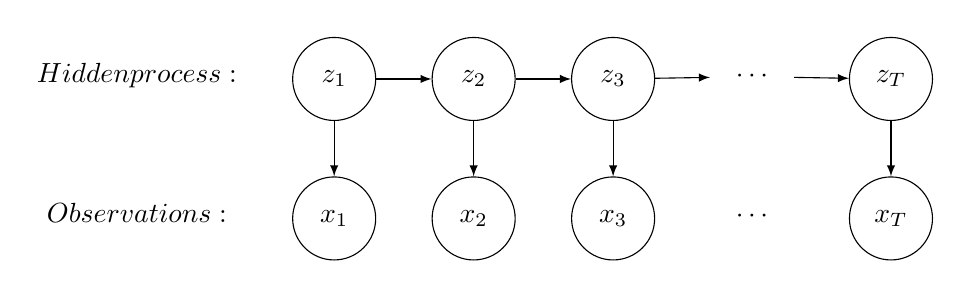
\begin{tikzpicture}
			\matrix[matrix of math nodes,column sep=2em,row
			sep=2em,cells={nodes={circle,draw,minimum width=3em,inner sep=0pt}},
			column 1/.style={nodes={rectangle,draw=none}},
			column 5/.style={nodes={rectangle,draw=none}}] (m) {
				\text{Hidden process}: &
				z_1 & z_2 & z_3 & \cdots & z_T\\
				\text{Observations}: & 
				x_1 & x_2 & x_3 & \cdots & x_T\\
			};
			\foreach \X in {2,3,4,5}
			{\draw[-latex] (m-1-\X) -- (m-1-\the\numexpr\X+1) node[midway,above]{};
				\ifnum\X=5
				\draw[-latex] (m-1-6) -- (m-2-6) node[pos=0.6,left]{};
				\else
				\draw[-latex] (m-1-\X) -- (m-2-\X) node[pos=0.6,left]{};
				\fi}
		\end{tikzpicture}
		\caption{Dependency graph of an HMM}
	\end{figure}
	
	\subsection{The Full Model Joint Distribution}
	Given a set of model parameters $\lambda=(A,B,\pi)$, the full joint distribution $p(\mathcal{X},\mathcal{Z})$ can be written in a clean, intuitive form by conditioning on the hidden state sequence $ p(\mathcal{X},\mathcal{Z}) = p(\mathcal{X}|\mathcal{Z}) p(\mathcal{Z}) $.
	The conditional distribution is easy to find since with every state known, the probability of each observation is determined by the corresponding measurement distribution. Indeed, we have 
	$$p(\mathcal{X}|\mathcal{Z}) = \prod_{t=1}^T b_{z_t}(x_t)$$ Meanwhile the hidden sequence distribution $p(\mathcal{Z})$ can be found by iteratively conditioning on all previous times with $p(\mathcal{Z})=p(z_T|z_{1:T-1})p(z_{1:T-1})$. Iterating this back to the beginning, we find the distribution is 
	$$p(\mathcal{Z}) = \pi_{z_1}\prod_{t=2}^T A_{z_tz_{t-1}}$$ This is understood in simple terms --- the probability of a hidden sequence $z_1\dots z_T$ is the probability of $z_1$ (i.e. $\pi_{z_1}$) multiplied by the transition probability to $z_2$ multiplied by the transition probability to $z_3$, on and on until we get to the end of the sequence. Combining these findings, the full joint distribution $p(\mathcal{X},\mathcal{Z}) = p(\mathcal{X}|\mathcal{Z})p(\mathcal{Z})$ is the product of probabilities:
	$$ p(\mathcal{X},\mathcal{Z}) = \pi_{z_1}b_{z_1}(x_1) \prod_{t=2}^T A_{z_tz_{t-1}}b_{z_t}(x_t)$$
	This joint distribution is central to this note since from it, we will be able to compute any probability we like.
	
	
	\section{Observation Probability}
	\subsection{Probability of an Observed Sequence}
	Given an observed sequence $\mathcal{X}$ and a set of model parameters $\lambda = (A,B,\pi)$, what is the probability of those observations $p(\mathcal{X})$ given the model? With the full joint distribution $p(\mathcal{X},\mathcal{Z})$ in hand, answering this question amounts to simply marginalizing over all possible hidden sequences: $p(\mathcal{X})=\sum_{\mathcal{Z}}p(\mathcal{X},\mathcal{Z})$. More explicitly, we can write
	$$ p(\mathcal{X}) = \sum_{z_1\dots z_T}\pi_{z_1}b_{z_1}(x_1) \prod_{t=2}^TA_{z_tz_{t-1}}b_{z_t}(x_t) $$
	Seeing as there are $N^T$ possible hidden sequences and for each possible sequence we must multiply $2T$ factors, computing this likelihood by naively applying this formula requires $O(N^T T)$ operations. The exponential complexity is prohibitively demanding in an applied setting so a more computationally efficient approach is needed. The solution is known as the \emph{forward algorithm}.
	\subsection{The Forward Algorithm}
	The basic insight of the forward algorithm is that the naive computation of $p(\mathcal{X})$ is highly redundant. For example, we do not need to compute $\pi_n b_n(x_1)$ for all $N^T$ possible sequences. It can computed once and then used for all the others. To see how this works, we can simply rewrite the sums over the hidden states so that they include only the relevant terms. The result looks like:
	$$ p(\mathcal{X}) = \sum_{ z_T}\underbrace{b_{z_T}(x_T) \sum_{z_{T-1}}A_{z_Tz_{T-1}} \underbrace{b_{z_{T-1}}(x_{T-1})\dots \underbrace{b_{z_3}(x_3)\sum_{z_2}A_{z_3z_2} \underbrace{b_{z_2}(x_2)\sum_{z_1}A_{z_2z_1}\underbrace{b_{z_1}(x_1)\pi_{z_1}}_{\alpha_{z_1,1}}}_{\alpha_{z_2,2}}}_{\alpha_{z_3,3}}}_{\alpha_{z_{T-1},T-1}}}_{\alpha_{z_T,T}}$$
	Here we have defined each incremental sum by the \textbf{forward probability} $\alpha_{m,t}\equiv p(x_{1:t},z_t=m)$. Looking closely at the above dissected equation, one finds that the forward probabilities satisfy a recursion relation:
	$$ \alpha_{m,t} = b_m(x_t) \sum_n A_{mn} \alpha_{n,t-1}$$
	which has as a base case $\alpha_{m,1}=b_m(x_1)\pi_m$. If there is any uncertainty that the forward probabilities are in fact $p(x_{1:t}, z_t)$, one can marginalize over $z_{t-1}$ to quickly find this same recursion formula. To emphasize:
	$$ \alpha_{m,t} \equiv \t{likelihood of observing $x_{1:t}$ and ending up in state $z_t=m$} $$
	
	To compute $p(\mathcal{X})$, we can iterate this recursive formula to compute the forward probability at any time. To compute $\alpha_{m,t}$ for all $N$ possible states at time $t$ requires computing the above $N$-term sum $N$ times. So iterating this up to time $T$ takes $O(N^2T)$ operations --- a dramatic improvement on the time complexity of our calculation. Finally, with an additional $N$-term sum, we obtain the observation likelihood with 
	$$ p(\mathcal{X}) = \sum_m\alpha_{m,T} $$
	Introducing the vector notation $\*b(x_t)\equiv(b_1(x_t)\dots b_N(x_t))$ and $\*\pi=(\pi_1\dots\pi_N)$, calculating the forward probabilities can be implemented in a vectorized form using a Hadamard product and a matrix multiplication:
	
	\begin{algorithm}
		\caption{Forward Algorithm --- Vectors}
		\SetKwInOut{Input}{Input}
		\SetKwInOut{Output}{Output}
		
		\underline{function Forward}$(\mathcal{X},\lambda)$\\
		\Input{$\mathcal{X}$, $\lambda=(A,B,\pi)$}
		\Output{$N\times T \t{ matrix of forward probabilities } \alpha$}
		$\alpha \leftarrow 0_{N\times T}$
		
		$\alpha[:,1] \leftarrow \*b(x_1)\odot \*\pi$
		
		\For{$t=2 \t{ to } T$}{
			$\alpha[:,t] \leftarrow  \*b(x_t)\odot A\alpha[:,t-1]$
		}
		
		return $\alpha$
	\end{algorithm}
	
	\subsection{The Backward Algorithm}
	The forward algorithm begins at the beginning $t=1$ and then works its way forward in time, computing possible paths in the hidden state space. Alternatively, one can work backward. The sum of all the hidden states can be done in the opposite order as made clear by writing the equation as
	$$p(\mathcal{X}) = \sum_{z_1}\pi_{z_1}b_{z_1}(x_1)
	\underbrace{\sum_{z_2}A_{z_2z_1}b_{z_2}(x_2)
		\underbrace{\sum_{z_3}A_{z_3z_2}b_{z_3}(x_3)\dots \underbrace{\sum_{z_{T-1}}A_{z_{T-1}z_{T-2}}b_{z_{T-1}}(x_{T-1})
				\underbrace{\sum_{z_T}A_{z_Tz_{T-1}}{b_{z_T}(x_T)}}_{\beta_{z_{T-1},T-1}}}_{\beta_{z_{T-2},T-2}}}_{\beta_{z_2,2}}}_{\beta_{z_1,1}}$$
	The \textbf{backward probability} $\beta_{n,t}\equiv p(x_{t+1:T}|z_t=n)$ satisfies a \emph{backwards} recursive equation which can be read off from the above to write
	$$ \beta_{n,t} = \sum_m A_{mn} b_m(x_{t+1})\beta_{m,t+1} $$
	To work with the equation for $p(\mathcal{X})$, we must take the base case $\beta_{n,T}=1$ for all $n=1\dots N$. To emphasize, the interpretation of the backward probabilities is
	$$ \beta_{n,t} \equiv \t{likelihood of observing $x_{t+1:T}$ given the preceding state was $z_t=n$ } $$
	Applying the recursion and eventually getting back to $\beta_{n,1}$, the observation probability is computed as
	$$ p(\mathcal{X}) = \sum_n\pi_nb_n(x_1)\beta_{n,1} $$
	The backwards algorithm runs in $O(N^2T)$ time just like the forward algorithm. Similar to before, it can be vectorized so that the algorithm is:
	
	\begin{algorithm}
	\caption{Backward Algorithm --- Vectors}
	\SetKwInOut{Input}{Input}
	\SetKwInOut{Output}{Output}
	
	\underline{function Backward}$(\mathcal{X},\lambda)$\\
	\Input{$\mathcal{X}$, $\lambda=(A,B,\pi)$}
	\Output{$N\times T\t{ matrix of backward probabilities } \beta$}
	
	$\beta \leftarrow 0_{N\times T}$
	
	$\beta[:,T] \leftarrow (1\dots 1) \in \R^N$
	
	\For{$t=T-1 \t{ down to } 1$}{
		$\beta[:,t] \leftarrow  (\*b(x_{t+1})\odot \beta[:,t+1])A$
	}
	
	return $\beta$
\end{algorithm}
	
	\section{Inference of Hidden States}
	\subsection{Distribution of $z_t$ --- The Forward-Backward Algorithm}
	So then, the forward and backward algorithms provide two different efficient ways to compute the observation probability $p(\mathcal{X})$. But ultimately, these two algorithms will turn out to be complementary rather than alternatives of one another. They can be used together to compute other quantities that will be very important to inference with HMMs. Crucially, consider the following question: given an observation sequence $\mathcal{X}$ and model parameters $\lambda=(A,B,\pi)$, what is the distribution of the hidden state $z_t$? In other words, what is the distribution $p(z_t|\mathcal{X})$? This probability can be written in terms of the forward and backward probabilities opening up the possibility of using both the forward and backward algorithms. 
	$$ p(z_t=m|\mathcal{X})=\frac{p(\mathcal{X},z_t=m)}{p(\mathcal{X})} = \frac{\overbrace{p(x_{t+1:T}|z_t=m)}^{\beta_{m,t}}\overbrace{p(x_{1:t},z_t=m)}^{\alpha_{m,t}}}{p(\mathcal{X})} $$	
	In the second equality, the observation sequence is split into times up to $t$ and then all future times to $T$: $\mathcal{X}=(x_{1:t}, x_{t+1:T})$. The denominator is a simple normalizing factor in this case and we can write
	$$ p(z_t=m|\mathcal{X}) = \frac{\beta_{m,t}\alpha_{m,t}}{\sum_{n=1}^N \beta_{n,t}\alpha_{n,t}} $$
	So, in order to calculate the distribution for the state at time $t$, we can use both the forward and backward algorithms to recursively compute $\alpha_{m,t}$ and $\beta_{m,t}$. With these, the distribution is found through the above equation. 
	
	\subsection{Distribution of $(z_t,z_{t-1})$}
	Another important distribution for training HMMs on real data is for consecutive states $p(z_t=m,z_{t-1}=n|\mathcal{X})$. Similar to before, we split the set of observations as $\mathcal{X}=(x_{1:t-1}, x_t, x_{t+1:T})$ and then the chain rule gives:
	$$p(z_t=m,z_{t-1}=n|\mathcal{X}) = \frac{p(x_{t+1:T}|z_t=m)p(x_t|z_t=m)p(z_t=m|z_{t-1}=n)p(x_{1:t-1},z_{t-1}=n)}{p(\mathcal{X})}$$
	Identifying the known distributions appearing in this expression, we can write more compactly:
	$$ p(z_t=m,z_{t-1}=n|\mathcal{X}) = \frac{\beta_{m,t}b_m(x_t)A_{mn}\alpha_{n,t-1} }{\sum_{\mu,\nu=1}^N \beta_{\mu,t}b_\mu(x_t)A_{\mu\nu}\alpha_{\nu,t-1} } $$
	
	\subsection{Most Probable State Sequence --- The Viterbi Algorithm}
	Now consider another question: given an observation sequence $\mathcal{X}$ and model parameters $\lambda=(A,B,\pi)$, what is the most probable sequence of hidden states $\mathcal{Z}$? More formally, the problem may be written as $ \hat{\mathcal{Z}} = \arg\max_\mathcal{Z} p(\mathcal{Z}|\mathcal{X}) $. However since the conditional distribution is related to the joint distribution through $p(\mathcal{X},\mathcal{Z})=p(\mathcal{Z}|\mathcal{X})p(\mathcal{X})$ and the observation sequence is fixed, we will write the problem more conveniently as
	$$\hat{\mathcal{Z}}=\arg\max_\mathcal{Z} p(\mathcal{X},\mathcal{Z})$$
	Naively, there are $N^T$ possible paths of length $T$ through state space. The exponential number makes brute force maximization computationally infeasible, so a more clever algorithm is needed. The solution to this problem can be found through \textbf{dynamic programming}. Suppose we know the probability of the most likely state sequence up to time $t$ that ends in state $n$, i.e.
	$$ \delta_{m,t} \equiv \max_{z_{1:t-1}} p(x_{1:t}, z_{1:t-1}, z_t=m) $$
	This has a recursive structure that can be exploited. Observe that this distribution can be factored by conditioning on $x_t, z_t,$ and $z_{t-1}$ to find $p(x_{1:t}, z_{1:t-1}, z_t)=p(x_{1:t-1}, z_{1:t-2})p(x_t|z_t)p(z_t|z_{t-1})$. From this form, the maximization over $z_{t-1}$ can be isolated from the other $z_{1:t-2}$ and the recursive structure is revealed:
	$$ \delta_{m,t} \equiv b_m(x_t) \max_n \left[ A_{mn} \delta_{n,t-1} \right] $$
	At $t=1$, this is simply $\delta_{n,1}=b_n(x_1)\pi_n$. If this recursion is taken to the end of the time series, then we have $\delta_{n,T}$ which is by definition the probability that the most likely sequence ends in state $n$. So $\arg\max_n \delta_{n,T} $ is the final state of the most likely sequence. With this, we can perform a backtrace to construct the full state sequence $\hat{\mathcal{Z}}$. Observe that $\psi_{m,t} = \arg\max_n [A_{mn}\delta_{n,t-1}]$ is the 

	
	\begin{algorithm}
	\caption{Viterbi Algorithm --- Vectors}
	\SetKwInOut{Input}{Input}
	\SetKwInOut{Output}{Output}
	
	\underline{function Viterbi}$(\mathcal{X},\lambda)$\\
	\Input{$\mathcal{X}$, $\lambda=(A,B,\pi)$}
	\Output{$\t{Most probable state sequence } \hat{\mathcal{Z}}$}
	
	$\delta \leftarrow 0_{N\times T}$
	
	$\psi \leftarrow 0_{N\times T}$
	
	$\delta[:,1] \leftarrow \*b(x_1)\odot\*\pi$
		
	\For{$t=2 \t{ to } T$}{
		\For{$m=1 \t{ to } N$}{
		$y \leftarrow A[m,:]\odot \delta[:,t-1] $
		
		$ \delta[m,t] \leftarrow  b_m(x_t)\; \max y$
		
		$\psi[m,t] \leftarrow \arg\max y  $
	}
	}
	
	$\hat{\mathcal{Z}} \leftarrow (0\dots 0)\in\R^T$
	
	$ \hat{\mathcal{Z}}[T] = \arg\max \delta[:,T] $
	
	\For{$t=T-1 \t{ down to }$ 1}{
		$\hat{\mathcal{Z}}[t] = \psi[\hat{\mathcal{Z}}[t+1], t+1 ]$
	}
	
	
	return $\hat{\mathcal{Z}}$
\end{algorithm}

	
	\section{HMM Learning}
	\subsection{The Baum-Welch Algorithm}
	Suppose we have some set of observations $\mathcal{X}$ and we wish to estimate the HMM parameters $\lambda=(A,B,\pi)$. The standard approach to this problem is to compute a maximum-likelihood estimator via the EM algorithm (known in this context as the \textbf{Baum-Welch algorithm}). Recall the EM algorithm is iterative, eventually converging to a local maximum in the likelihood function through a sequence of expectation calculations and maximizations. The iteration rule is
	$$ \hat\lambda^{i+1}=\arg\max_\lambda Q(\lambda|\hat\lambda^i) \qquad\qquad Q(\lambda|\hat\lambda^i)\equiv \mathbb{E}_{\mathcal{Z}|\mathcal{X},\hat\lambda^i}[\log p(\mathcal{X},\mathcal{Z}|\lambda)]$$
	The expectation can be computed as
	$$ Q(\lambda|\hat\lambda^i) = \sum_\mathcal{Z} \gamma^i(\mathcal{Z})\log p(\mathcal{X},\mathcal{Z}|\lambda) $$
	where the sum is over all possible hidden state sequences $\mathcal{Z}$ and the probability of a particular state sequence given the current parameter estimates is denoted $\gamma^i(\mathcal{Z})\equiv p(\mathcal{Z}|\mathcal{X},\hat\lambda^i)$. To apply the EM algorithm to find HMM parameters, we can use the form for the HMM joint distribution found previously. Taking its logarithm, the $Q$ function takes the following form
	$$ Q(\lambda|\hat\lambda^i) = \sum_{\mathcal{Z}}\gamma^i(\mathcal{Z})\left[\log\pi_{z_1} + \sum_{t=1}^T\log b_{z_t}(x_t) + \sum_{t=2}^T \log A_{z_tz_{t-1}}\right] $$
	The sum over hidden sequences can be simplified by bringing it inside the sums over time in which only one or two hidden states will be relevant for each time. The rest of the sums simply marginalize $\gamma^i(\mathcal{Z})$ leaving a simpler, albeit time-dependent, probability in its place. Using the notation $\gamma^i(\cdot) = p(\cdot|\mathcal{X},\hat\lambda^i)$, we may just note that $\gamma^i(z_t)$ is the marginalization of $\gamma^i(\mathcal{Z})$ over all $z_\tau$ for $\tau\neq t$. Similarly $\gamma^i(z_t,z_{t-1})$ is the marginalization over all $z_\tau$ except for $\tau\in\{t,t-1\}$. With this, we have a more palatable objective function to maximize:
	$$ Q(\lambda|\hat\lambda^i) = \sum_{z_1}\gamma^i(z_1)\log\pi_{z_1} + \sum_{t=1}^T\sum_{z_t}\gamma^i(z_t)\log b_{z_t}(x_t) + \sum_{t=2}^T \sum_{z_t}\sum_{z_{t-1}}\gamma^i(z_t,z_{t-1}) \log A_{z_tz_{t-1}} $$
	To now maximize this, we must use Lagrange multipliers to constrain the solution to satisfy the probabilistic sum rules. Namely, the initial state distribution is normalized $\sum_n \pi_n =1$, the transition probabilities are normalized so that transitioning to \emph{any} state has probability $\sum_mA_{mn}=1$, and finally the measurement probabilities must be normalized so that\footnote{The measurements could be discrete or continuous. In the discrete case, the pdf has the form $b_n(x)=\sum_{m}B_{mn}\delta(x-m)$} $\int dx\;b_n(x)=1$ for any hidden state $n=1\dots N$. The Lagrangian we want is given by
	$$ \mathscr{L}(\lambda|\hat\lambda^i) = Q(\lambda|\hat\lambda^i) - \eta_\pi\sum_{n=1}^N \pi_n - \sum_{n=1}^N \eta_{A,n} \sum_{m=1}^N A_{mn} - \sum_{n=1}^N \eta_{B,n} \int dx\;b_n(x) $$
	where $\eta_{\bullet,n}$ are the Lagrange multipliers. Finding the stationary points with respect to each parameter, we can derive the update equations needed to implement the M-step of the EM algorithm. For the initial state distribution, we find that $\frac{\partial\mathscr{L}}{\partial \pi_n}=0$ yields the solution $\pi_n^{i+1}=\gamma^i(z_1=n)/\eta_\pi$ and similarly, for each element of the transition matrix we find that $\frac{\partial\mathscr{L}}{\partial A_{mn}}=0$ yields $A_{mn}^{i+1}=\sum_{t=2}^T \gamma^i(z_t=m,z_{t-1}=n)/\eta_{A,n}$. The multipliers $\eta_\pi$ and $\eta_{A,n}$ are found by enforcing the normalization conditions and therefore these are simple normalization constants. Through that normalization, we find the full update equations:
	\begin{align*}
		\pi_n^{i+1} &= \gamma^i(z_1=n) \\
		A_{mn}^{i+1} &= \frac{\sum_{t=2}^T \gamma^i(z_t=m,z_{t-1}=n) }{\sum_{t=2}^T\gamma^i(z_{t-1}=n)}
	\end{align*}
	The measurement probabilities are more flexible in HMMs so must be given more attention than the initial distribution and transition probabilities. 
	\subsubsection{Discrete Categorical Measurements}
	In the simplest scenario where the observations are discrete-valued and their distribution is totally non-parametric, we define a measurement matrix $B_{mn}\equiv p(x_t=m|z_t=n)$ which is normalized through $\sum_m B_{mn}=1$. The stationary points of the Lagrangian found through $\frac{\partial \mathscr{L}}{\partial B_{mn}}=0$ are
	$$B_{mn}^{i+1} = \frac{\sum_{t|x_t=m}\gamma^i(z_t=n)}{\sum_{t=1}^T\gamma^i(z_t=n)}$$
	where take note that the sum is over times only where the observation was $m$. 

	\subsubsection{Gaussian Measurements}
	Alternatively, it is popular to use a state-dependent parametric model for our observations. As an important example, suppose each state corresponds to a different normal distribution so that state transitions simply correspond to a shift in mean and/or variance. More generally, we will consider the multivariate case where $x_t\in\R^M$ and each state $n$ corresponds to a measurement distribution $\mathcal{N}(\mu_n,\Sigma_n)$. With this model for the measurements, the normalization is baked into the standard multivariate normal pdf so the Lagrangian simplifies to just $ \mathscr{L}(\lambda|\hat\lambda^i) = \dots - \frac{1}{2}\sum_{t=1}^T \sum_{z_t} \gamma^i(z_t) (x_t- \mu_{z_t})^\t{T}\Sigma_{z_t}^{-1}(x_t- \mu_{z_t})+ \dots  $ where we have focused on only the relevant term.
	Finding stationary points, one can derive the following  update rules
	\begin{align*}
		\hat\mu^{i+1}_n = \frac{\sum_{t=1}^T	 \gamma^i(z_t=n)x_t}{\sum_{t=1}^T \gamma^i(z_t=n)}&&
		\hat\Sigma_n^{i+1} = \frac{\sum_{t=1}^T\gamma^i(z_t=n)(x_t - \hat\mu_n^{i+1})(x_t - \hat\mu_n^{i+1})^\t{T}}{\sum_{t=1}^T \gamma^i(z_t=n)}
	\end{align*}
	Observe that these update equations exactly match those used for a Gaussian mixture model (GMM) which assigns each data point to one of $N$ normal distributions. This is in effect exactly what the Gaussian HMM is doing --- it finds $N$ Gaussians which best capture the data. However, a GMM has nothing to say about the \emph{sequential} features in the data. In contrast, an HMM models the sequential nature of the data through the Markov process and its transition probabilities. 
	
	In general, we can assume any measurement distribution and update its parameters iteratively like this. In the worst case scenario, no closed form update rule can be found so a numeral maximization must be performed. 
	
	
	\section{Constrained Models}
	\subsection{HMMs as Directed Weighted Graphs}
	Without placing any constraints on the transition matrix $A$, the set of all hidden states $1\dots N$ is \textbf{fully connected} --- every possible transition is allowed with some probability. This is not always desired. For example, suppose an HMM is being used to model a system with a \emph{terminal} state that can be reached by other states, but once in it, the system remains in it forever. This constrains the model so that the only transition from the terminal state is back to itself. In terms of the transition matrix, we require that the column of $A$ corresponding to transitions from the terminal state has only one nonzero entry: the diagonal element.
	
	In general, the state transitions can be constrained in any arbitrary way. Mathematically, the set of hidden states and transitions between them form a \textbf{directed graph}. The vertices of the graph are the states and the edges represent transitions. Note that any such graph can be obtained by pruning the fully connected graph so that all the forbidden transitions are removed. Practically speaking, this amounts to setting the corresponding element of the transition matrix to zero: $A_{mn}=0$. Note that by using the forward-backward algorithm to compute $\gamma^i(z_t,z_{t-1})$ for the update, if $A_{mn}=0$ at the beginning, then it will remain zero after each update.  The inter-state connections define the \textbf{topology} of the hidden state space.
	
	
	
	\section{Hidden Semi-Markov Models (HSMM)}
	\subsection{State Duration (a.k.a. Sojourn Time)}
	One of the greatest limitations of the standard HMM is how it models \emph{state duration}. Consider the probability of being in state $n$ for $\ell$ consecutive time steps. This amounts to an initial $n$-state followed by $\ell-1$ transitions to itself followed by a final transition to any other state. Translating this into an equation looks like
	$$ p(\ell|z_t=n)= A_{nn}^{\ell-1}(1 - A_{nn}) $$
	Therefore the HMM implicitly assumes that the state duration is geometrically/exponentially distributed. Shorter state durations are always more probable than longer ones. 
	
	Work has been done to address this limitation and higher order models have been constructed that allow for more generic distributions for the state duration. The most notable model is the \textbf{hiddden semi-Markov model} (HSMM).
	
	\subsection{Introduction to HSMMs}
	Like an HMM, an HSMM consists of a sequence of observations $\mathcal{X}$ along with a hidden sequence of states $\mathcal{Z}$. The difference is that in an HSMM, each state can emit several observations instead of just one. To make this work, we must change how we index our states vs our observations. Whereas the observations remain indexed by the real-time values $t=1\dots T$, the states will be indexed by their \textbf{time segment} corresponding to a sequence of times where the state does not change. Each time segment $s$ has a corresponding sequence of observations $\mathcal{X}_s$ with start time $t_s^\star$ and a duration $\ell_s$ so that
	$$ \mathcal{X}_s = (x_{t_s^\star}\; \dots\; x_{t_s^\star+\ell_s-1} )$$
	The model is ``semi-Markov" because the state dynamics are only Markovian at the segment boundaries. Formally, this means that the state sequence is Markovian in terms of the segment index $s$, but \emph{not} the time value $t$. 
	
		\begin{figure}[b!]
		\centering
		\begin{tikzpicture}
			\matrix[matrix of math nodes,column sep=2em,row
			sep=2em,cells={nodes={circle,draw,minimum width=3em,inner sep=0pt}},
			column 1/.style={nodes={rectangle,draw=none}},
			column 5/.style={nodes={rectangle,draw=none}}] (m) {
				\text{Hidden process}: &
				z_1 & z_2 & z_3 & \cdots & z_L\\
				\text{Observations}: & 
				\t{ }x_{t_1^\star:t_1^\star+\ell_1-1} & \t{ }x_{t_2^\star:t_2^\star+\ell_2-1} & \t{ }x_{t_3^\star:t_3^\star+\ell_3-1} & \cdots & \t{ }x_{t_L^\star:T}\\
			};
			\foreach \X in {2,3,4,5}
			{\draw[-latex] (m-1-\X) -- (m-1-\the\numexpr\X+1) node[midway,above]{};
				\ifnum\X=5
				\draw[-latex] (m-1-6) -- (m-2-6) node[pos=0.6,left]{};
				\else
				\draw[-latex] (m-1-\X) -- (m-2-\X) node[pos=0.6,left]{};
				\fi}
		\end{tikzpicture}
		\caption{Dependency graph of an HSMM. Each state $z_s$ emits a sequence of observations with a random length $\ell_s$. The states and observations are no longer 1-to-1.}
	\end{figure}
	
	Just as with the HMM, we will now derive the full joint density of the model so that more refined values can be obtained from it. To start, note that there is now an additional random variable associated with each state: its duration. If $\mathcal{L}=(\ell_1 \dots \ell_L)$ denotes a set of segment durations, then the full joint density can be factored as
	$$ p(\mathcal{X}, \mathcal{Z}, \mathcal{L}) =p(\mathcal{X}|\mathcal{Z},\mathcal{L})p(\mathcal{Z},\mathcal{L})$$
	The probability of a given hidden sequence $\mathcal{Z}$ with durations $\mathcal{L}$ can be derived similar to before to write
	$ p(\mathcal{Z},\mathcal{L}) = \pi_{(z_1,\ell_1)} \prod_{s=2}^L A_{(z_s,\ell_s)(z_{s-1},\ell_{s-1})} $. Maintaining the assumption that all observations only depend on their current state, we have the full joint distribution for an HSMM:
	$$ p(\mathcal{X},\mathcal{Z},\mathcal{L}) = \pi_{(z_1,\ell_1)}p(\mathcal{X}_1|z_1,\ell_1)\prod_{s=2}^L A_{(z_s,\ell_s)(z_{s-1},\ell_{s-1})}p(\mathcal{X}_s|z_s,\ell_s)  $$
	Note that the transition probabilities are generally specified by transitions from a specified \emph{state and duration} to another \emph{state and duration}: $(z_{s-1},\ell_{s-1})\to(z_s,\ell_s)$. Consequently the effective number of states that the full transition matrix must account for is $NT$ ($T$ is the number of possible duration values) and so the matrix size grows quadratically with the length of the time-series. This is typically a huge computational burden even if we limit the maximum duration to some value $\ell_\t{max}\leq T$. The forward/backward algorithms for this general HSMM require $O(N^2\ell_\t{max}^2T)$ operations.
	
	It is worth pointing out that since the observations depend on the state as a full segment $\mathcal{X}_s$ rather than a single value $x_t$, there is opportunity to introduce some more complex dependencies in the observation sequence. For example, some popular model choices for within each segment include linear dynamical systems, autoregressive models, and even HMMs themselves.
	
	From the full joint distribution, the observation likelihood is  found by integrating over the hidden states and their corresponding durations: $p(\mathcal{X}) = \sum_\mathcal{Z}\sum_\mathcal{L}p(\mathcal{X},\mathcal{Z},\mathcal{L})$. More explicitly:
	$$ p(\mathcal{X}) = \sum_L\sum_{\ell_1\dots\ell_L}\mathbbm{I}_{\ell_1+\dots+\ell_L=T}\sum_{z_1\dots z_L} \:\pi_{(z_1,\ell_1)}p(\mathcal{X}_1|z_1,\ell_1)\prod_{s=2}^L A_{(z_s,\ell_s)(z_{s-1},\ell_{s-1})}p(\mathcal{X}_s|z_s,\ell_s) $$
	The marginalization over all possible durations $\mathcal{L}$ appears as $\sum_\mathcal{L} =\sum_L\sum_{\ell_1\dots\ell_L}\mathbbm{I}_{\ell_1+\dots+\ell_L=T}$ where $\mathbbm{I}$ is the indicator function so that all possible segmentations are considered subject to the contraint that $\sum_s \ell_s = T$. From here, forward and backward probabilities can be derived similar to was done for the basic HMM. With those values, inference and learning algorithms can be constructed.
	
	
	\section{Explicit Duration HMMs (EDHMMs)}
	\subsection{HSMMs With Renewal Structure}
	The general HSMM discussed so far is a powerful model but suffers from computational complexity due to the $N\ell_\t{max}$-dimensional state space. For practical application, some simplifying structure is usually needed. Perhaps the most common approach is to make the following two assumptions:
	\begin{itemize}
		\item Assume each state is independent of the previous duration, i.e. $p(z_s|z_{s-1},\ell_{s-1})=p(z_s|z_{s-1})$
		\item Assume each duration depends only on the simultaneous state, i.e. $p(\ell_s|z_s,z_{s-1},\ell_{s-1}) = p(\ell_s|z_s)$
	\end{itemize}
	Noting that the transition probabilities decompose as $p(z_s,\ell_s|z_{s-1},\ell_{s-1}) = p(\ell_s|z_s,z_{s-1},\ell_{s-1})p(z_s|z_{s-1},\ell_{s-1})$, these assumptions allow the large transition matrix to be factored so that:
	$$A_{(z_s,\ell_s),(z_{s-1},\ell_{s-1})} = q_{z_s}(\ell_s)A_{z_sz_{s-1}} $$
	where we now have an explicit duration distribution that will be denoted by $q_m(\ell)\equiv p(\ell_s=\ell|z_s=m)$. This can be modeled however we like so that different states have different duration characteristics. This simplified form of HSMM is called an \textbf{explicit duration HMM} (EDHMM).
	
	The EDHMM joint distribution is
	$$ p(\mathcal{X},\mathcal{Z},\mathcal{L}) = q_{z_1}(\ell_1)\pi_{z_1}  b_{z_1}(\mathcal{X}_1)\prod_{s=2}^L q_{z_s}(\ell_s) A_{z_sz_{s-1}} b_{z_s}(\mathcal{X}_s) $$
	Note that the final state's duration ought to be treated separately since the observations extend to time $T$, but there is not necessarily a state transition at that time. To avoid any extra assumptions, the sojourn probability at the last state can be modeled with a \textbf{survivor function}: 
	$$ p(\ell_L|z_L) \mapsto \sum_{\ell\geq \ell_L} p(\ell|z_L) $$
	
	\subsection{Forward and Backward Algorithms for EDHMMs}
	Similar to how it was done previously, the forward algorithm for EDHMMs can be derived by expanding out the sum for $p(\mathcal{X})$. By evaluating the sums forward in time, we find the forward probabilities $\alpha_{m,t}=p(x_{1:t}, z_t=m)$ satisfy the recursion relation
	$$ \alpha_{m,t} = \sum_{\ell=1}^{\min(t-1, \ell_\t{max})} b_m(x_{t-\ell_i+1:t}) q_m(\ell)\sum_n A_{mn} \alpha_{n,t-\ell} $$
	where the initial value is defined by the duration of the first state: $\alpha_{n,t}=b_n(x_{1:t})q_n(t)\pi_n$. Notice that by constraining the sum over durations at each time, the constaint that $\sum_i\ell_i=T$ is always satisfied by paths traversed in the sum. The observation likelihood is $p(\mathcal{X})=\sum_m\alpha_{m,T}$. The forward probabilities are then calculated with the following algorithm where the duration probability vector $\*q(\ell) = (q_1(\ell) \;\dots\;q_N(\ell))$ is defined for vectorization convenience.
	
	\begin{algorithm}
	\caption{EDHMM Forward Algorithm --- Vectors}
	\SetKwInOut{Input}{Input}
	\SetKwInOut{Output}{Output}
	
	\underline{function Forward}$(\mathcal{X},\lambda)$\\
	\Input{$\mathcal{X}$, $\lambda=(A,B,\pi,q,\ell_\t{max})$}
	\Output{$N\times T \t{ matrix of forward probabilities }\alpha$}
	$\alpha \leftarrow 0_{N\times T}$
	
	\For{$t=1 \t{ to } \ell_\t{max}$}{
	$\alpha[:,t] \leftarrow \*b(x_{1:t})\odot \*q(t) \odot \*\pi$
	}
	
	\For{$t=2 \t{ to } T$}{

	\For{$\ell=1 \t{ to } \min(t-1, \ell_\t{max})$}{

		$\alpha[:,t] \leftarrow \alpha[:,t] +   \*b(x_{t-\ell+1:t})\odot \*q(\ell)\odot A\alpha[:,t-\ell]$
	}}
	
	return $\alpha$
	\end{algorithm}

	Similarly a backward algorithm can be derived. The backward recursion for EDHMMs has the form
	$$ \beta_{n,t} = \sum_{\ell=1}^{\min(T-t,\ell_\t{max})} \sum_m q_m(\ell)A_{mn} b_m(x_{t+1:t+\ell})\beta_{m,t+\ell} $$
	where the base case is $\beta_{m,T} = 1$ for all final states $m$. The observation likelihood is calculated from the backward probabilities as $ p(\mathcal{X}) = \sum_{\ell}\sum_n\pi_n b_n(x_{1:\ell})\beta_{n,\ell} $. 
	
	\begin{algorithm}
	\caption{EDHMM Backward Algorithm --- Vectors}
	\SetKwInOut{Input}{Input}
	\SetKwInOut{Output}{Output}
	
	\underline{function Backward}$(\mathcal{X},\lambda)$\\
	\Input{$\mathcal{X}$, $\lambda=(A,B,\pi, q, \ell_\t{max})$}
	\Output{$N\times T \t{ matrix of backward probabilities } \beta$}
	$\beta \leftarrow 0_{N\times T}$
	
	$\beta[:,T] \leftarrow (1\dots 1) \in \R^N $
	
	\For{$t=T-1 \t{ down to } 1$}{
		\For{$\ell=1 \t{ to } \t{min}(T-t, \ell_\t{max})$}{
			$\beta[:,t] \leftarrow \beta[:,t] +  (\*q(\ell)\odot\*b(x_{t+1:t+\ell})\odot\beta[:,t+\ell])A$
	}
	}
	
	return $\beta$
	\end{algorithm}

	\section{Inference in EDHMMs}
		
	\section{EDHMM Learning}
	\subsection{Adaptation of the Baum-Welch Algorithm}
	The EM algorithm developed previously for training HMMs does not directly apply to HSMMs, but it can be adapted to work. The Q function in this case is defined by $Q(\lambda|\hat\lambda^i)\equiv \mathbb{E}_{\mathcal{Z},\mathcal{L}|\mathcal{X},\hat\lambda^i}[\log p(\mathcal{X},\mathcal{Z},\mathcal{L}|\lambda)]$, or more explicitly:
	$$ Q(\lambda|\hat\lambda^i) = \sum_{\mathcal{Z}}\sum_\mathcal{L}\gamma^i(\mathcal{Z},\mathcal{L})\left[\log\pi_{z_1} + \sum_{s=1}^L\log b_{z_s}(\mathcal{X}_s) + \sum_{s=2}^L \log A_{z_sz_{s-1}} + \sum_{s=1}^L\log p(\ell_s|z_s)\right] $$
	Proceeding just as before, we can bring in the sums over states/durations to write
	\begin{multline*} 
		Q(\lambda|\hat\lambda^i) = \sum_{z_1}\gamma^i(z_1)\log\pi_{z_1} +  \sum_{s=1}^L\sum_{z_s,\ell_s}\gamma^i(z_s,\ell_s)\log b_{z_s}(\mathcal{X}_s)  + \sum_{s=2}^L\sum_{z_s}\sum_{z_{s-1}}\gamma^i(z_s,z_{s-1}) \log A_{z_sz_{s-1}} \\+ \sum_{s=1}^L\sum_{z_s,\ell_s}\gamma^i(z_s,\ell_s)\log p(\ell_s|z_s)
	\end{multline*}
	where again $\gamma^i(\cdot) = p(\cdot|\mathcal{X},\hat\lambda^i)$. The derivative f
	
	\newpage
	\part*{Appendix}
	\appendix
	\section{Numerical Implementation}
	\subsection{Avoiding Underflow with Logarithms}
	In the forward and backward algorithms, many probabilities are multipled together to arrive at the final result and this can cause problems when implemented digitally. Considering that $0.1^{100} = 10^{-100}$, it is easy to imagine that we could run into \textbf{numerical underflows} fairly quickly with even a moderately sized dataset. Numerical underflows occur when a number is smaller than the smallest normal\footnote{A normal floating point number is one which has full precision since its exponent is being fully utilized. So for a single precision 8-bit exponent which takes values $-127$ to $127$, a number becomes subnormal when its exponent is saturated at $-127$ (all zero binary representation)} floating point representation and so precision is lost. For a single-precision float, the smallest positive normal number is $2^{-126}\approx 10^{-38}$. For double precision, it is $2^{-1022}\approx 10^{-308}$. So then if we are working with time-series data that has more than 308 time steps, then it is absolutely likely that we will run into numerical underflow problems. Any practical implementation of HMMs in code must address this issue.
	
	One standard approach is to perform all arithmetic on a logarithmic scale where even extreme numbers become manageable (e.g. $\log e^{-100} = -100$). Doing so, multiplication becomes simple addition ($\log ab = \log a + \log b$) but addition becoming more complex. To handle summing probabilities, we use the \textbf{logsumexp} operation which is based on the identity:
	$$\log(a+b) = \log(e^{\log a} + e^{\log b}) $$
	The intent here is to take the log-probabilities $\log a$ and $\log b$ as input and then perform the ``log of the sum of their exponents" to obtain $\log(a+b)$. Then to prevent possible overflows in the exponents, we factor out the max so that if $a>b$, we compute
	$$ \log(a+b) = \log a + \log(1 + e^{\log b  - \log a}) $$
	This ensure that the exponents are all non-positive so cannot overflow.
	
	In general, for a vector of log-probabilities $\*u=(u_1\dots u_M)$ such that $u_i=\log p_i$, we can compute the log of the probability sum with $\log(\sum_i p_i) = \t{logsumexp}(\*u)$ defined by 
	$$ \t{logsumexp}(\*u) \equiv \log u_\t{max} + \log\sum_ie^{u_i - u_\t{max}} $$
	where  $u_\t{max}\equiv \max_i u_i $. It is worth defining this as an algorithm:
	
	\begin{algorithm}
	\caption{logsumexp}
	\SetKwInOut{Input}{Input}
	\SetKwInOut{Output}{Output}
	
	\underline{function logsumexp}$(\*u)$\\
	\Input{$\*u\in \R^M \t{ such that } u_i=\log p_i$}
	\Output{$ \t{logsum} = \log(\sum_i p_i)$}
	$u_\t{max} \leftarrow  \max_i u_i$\\
	$\t{logsum} \leftarrow \log u_\t{max} + \log( \t{sum}( \exp(\*u-u_\t{max})))$
	
	return \t{logsum}
	\end{algorithm}
	\noindent This will be an essential ingredient in making the forward and backward algorithms numerically stable.
	\subsection{Numerically Stabilized Forward and Backward Algorithms}
	Consider now the standard forward recursion $\alpha_{m,t} = b_m(x_t)\sum_n  A_{mn}\alpha_{n,t-1}$. This can be written in terms of logs by using the logsumexp operation. We write
	$$ \log \alpha_{m,t} = \log b_m(x_t) + \t{logsumexp}(\log A_{m:} + \log \alpha_{:,t-1}) $$
	where the colon notation indicates all values in that index (i.e. $A_{m:}$ is the $m^\t{th}$ row of $A$). This yields the following numerically stable version of the forward algorithm:
	
	\begin{algorithm}
	\caption{Forward Algorithm --- Numerically Stable}
	\SetKwInOut{Input}{Input}
	\SetKwInOut{Output}{Output}
	
	\underline{function Forward}$(\mathcal{X},\lambda)$\\
	\Input{$\mathcal{X}$, $\lambda=(A,B,\pi)$}
	\Output{$N\times T \t{ matrix of forward log-probabilities } \alpha_\t{log} \equiv \log \alpha$}
	$\alpha_\t{log} \leftarrow 0_{N\times T}$
	
	$\alpha_\t{log}[:,1] \leftarrow \log\*b(x_1) + \log\*\pi$
	
	\For{$t=2 \t{ to } T$}{
		\For{$m=1 \t{ to } N$}{
			$\alpha_\t{log}[m,t] \leftarrow  \log b_m(x_t) +  \t{logsumexp}( \log A[m,:] + \alpha_\t{log}[:,t-1])$
		}
	}
	
	return $\alpha_\t{log}$
	\end{algorithm}
	
	We can similarly derive a numerically stable version of the backward algorithm. In this case, the recursion is 	$ \beta_{n,t} = \sum_m A_{mn} b_m(x_{t+1})\beta_{m,t+1} $ which, after taking logs, becomes
	$$ \log\beta_{n,t} = \t{logsumexp}\left( \log A_{:n} + \log\*b(x_{t+1}) + \log \beta_{:,t+1} \right) $$
	Writing this out as an algorithm, we have
	
	\begin{algorithm}
		\caption{Backward Algorithm --- Numerically Stable}
		\SetKwInOut{Input}{Input}
		\SetKwInOut{Output}{Output}
		
		\underline{function Backward}$(\mathcal{X},\lambda)$\\
		\Input{$\mathcal{X}$, $\lambda=(A,B,\pi)$}
		\Output{$N\times T\t{ matrix of backward log-probabilities } \beta_\t{log}$}
		
		$\beta_\t{log} \leftarrow 0_{N\times T}$
		
		\For{$t=T-1 \t{ down to } 1$}{
			\For{$n=1 \t{ to } N$}{
				$\beta_\t{log}[n,t] \leftarrow  \t{logsumexp}(\log A[:,n] + \log\*b(x_{t+1}) + \beta_\t{log}[:,t+1])$
			}
		}
		
		return $\beta_\t{log}$
	\end{algorithm}


	\section{Review of EM Algorithm}
	\subsection{Maximum Likelihood Estimation with Latent Variables}
	Consider an arbitrary model that has data $\mathcal{X}$, latent variables $\mathcal{Z}$, and parameters $\Theta$. A maximum likelihood estimation of the parameters works by maximizing over the marginal log-likelihood, i.e. the data likelihood: $$\hat\Theta=\arg\max_\Theta \log p(\mathcal{X}|\Theta) = \arg\max_\Theta \log\sum_\mathcal{Z} p(\mathcal{X},\mathcal{Z}|\Theta)$$ The problem we face is fitting the latent variables into this formulation. Since we have no data for those variables, they must be integrated out to obtain the data likelihood: $  p(\mathcal{X}|\Theta)  =\sum_{\mathcal{Z}} p(\mathcal{X},\mathcal{Z}|\Theta) $. The sum is over all possible values which is generally infeasible so a more efficient approach is needed. 
	
	The EM algorithm can be motivated in the following way. Suppose we have some guess for the parameters $\hat\Theta$. This would allow us to make some kind of inference about the latent variables through a distribution $p(\mathcal{Z}|\mathcal{X},\hat\Theta)$. Thinking of as the latent variables as missing data, then we can use the inferred distribution on $\mathcal{Z}$ to make a best guess at filling that missing data. More specifically, we can form a best guess at the full joint log-likelihood function $Q(\Theta)\equiv \log p(\mathcal{X},\mathcal{Z}|\Theta)$ by averaging over the latent variables. The expectation for the joint log-likelihood function is defined and denoted by $\hat Q(\Theta|\hat\Theta) \equiv \mathbb{E}_{\mathcal{Z}|\hat\Theta}\left[ \log p(\mathcal{X},\mathcal{Z} |\Theta) \right]$ is
	$$ \hat Q(\Theta|\hat\Theta) = \sum_{\mathcal{Z}} \underbrace{p(\mathcal{Z}|\mathcal{X},\hat\Theta)}_{\t{infer using $\hat\Theta$}} \log p(\mathcal{X},\mathcal{Z}|\Theta) $$
	With this best guess for the full likelihood function, we can then perform usual maximum likelihood estimation and compute a new estimate for the parameters: $ \hat\Theta \leftarrow \arg\max_\Theta \hat Q(\Theta|\hat\Theta)$. With these new parameters, we can repeat the same process to obtain an even better estimate for the latent variables and in turn a better estimate for the parameters. The EM algorithm is therefore iterative in nature with the rule
		$$ \hat\Theta^{t+1} = \arg\max_\Theta \hat Q(\Theta|\hat\Theta^t)$$


	
\end{document}